
\section{Imaging of Brain Activation}

The metabolic changes associated with the hemodynamic response can be accentuated through the use of fMRI \cite{Glover2011}. The following section will introduce the concept of fMRI and why it can be used to study brain activation. Before reading this section, it is assumed that the reader is familiar with basic physics of nuclear magnetic resonance imaging and image reconstruction. If not, an overview can be found appendices \ref{sec:physics} and \ref{sec:IMrec}. \\
The fundamental reason behind why fMRI can be used to study brain activity relies on the indirect measure of the magnetic properties of blood. MRI is dependent on susceptibility, which is the extend to which a material can be affected by magnetization. Local changes in susceptibility results in changes in the MR signal. \cite{Syed2015} Changes in susceptibility arise with the hemodynamic response as oxygenated hemoglobin $(HbO_2)$ is diamagnetic, and de-oxygenated hemoglobin $(Hb)$ is highly paramagnetic due to its four unpaired electrons, resulting in what is known as the Blood Level Oxygen Dependent (BOLD) contrast. Thus, as presented in the prior section, the increase in neural activity increases the blood flow to an extend greater than the metabolic utilization of oxygen, which results in a high $(HbO_2)$ to $(Hb)$ ratio. This makes up the difference in BOLD contrast. \cite{Glover2011,Poldrack2011,Khanna2015} \Figref{fig:back:bold} illustrates how the BOLD contrast is dependent on the amount of oxygenated hemoglobin. 

\begin{figure}[H]                 
	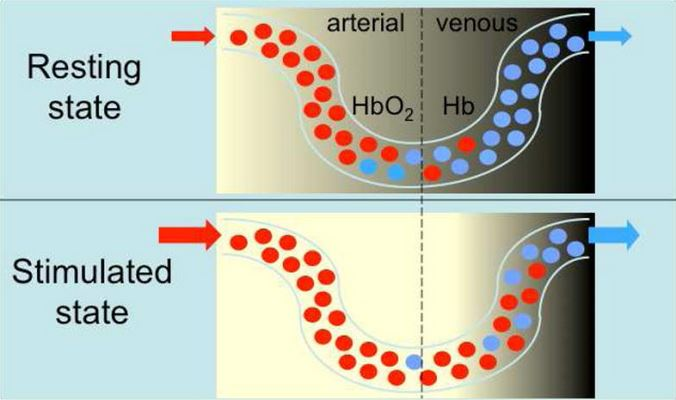
\includegraphics[width=.47\textwidth]{figures/aBackground/bold_response}  
	\caption{Illustration of the concentration difference in oxygenated $(HbO_2)$ and de-oxygenated hemoglobin $(Hb)$ during resting state and stimulated state. The diamagnetic properties of oxygenated blood changes the local magnetic substitutability facilitating a greater contrast change. \cite{Glover2011}}
	\label{fig:back:bold} 
\end{figure}

The changes in the BOLD contrast can be recorded by using a $T_{2}^*$ sequence, which is sensitive in detecting changes on the magnetic field \cite{Khanna2015,Lee2002}. The areas highly filled with oxygenated blood will result in a higher signal in the $T_{2}^*$-weighted sequence making these appear brighter in the reconstructed image. To capture the changes in blood flow over time the acquisitions has to be relatively fast. To achieve fast sequences, the result is a sacrifice of spatial resolution for temporal resolution, making it possible to acquire a whole brain volume in a couple of seconds. \cite{Khanna2015} \\ 
Other methods, as the arterial spin labeled (ASL) method exist for accentuating the functionality of the brain, but BOLD is favored, because it offers a high contrast to noise ratio and it is relatively simple to implement. \cite{Lee2002} \\ As fMRI can capture the neurological response to pain through the hemodynamic response a measure to study the individual's response to pain is thereby derived. To know more of how the individual's perception of pain is measured in general and by fMRI, including the current difficulties, is of great significance.    
